\newpage
\section{Anwendbarkeit von Business Intelligence auf Kryptomining Rechenzentren} \label{toc:ansatzmoeglichkeitenfuerbusinessintelligence}

In diesem Kapitel wird die Anwendbarkeit der Prinzipien von \ac{BI} Prozessen auf Kryptomining Rechenzentren geprüft, um eine
finanzielle Optimierung der Rechenzentren zu erreichen. Ziel dieses Teils ist die Prüfung der in Kapitel
\ref{toc:hypothesenundabgrenzungderarbeit} formulierten Teilhypothesen. Damit ist es möglich, letztendlich eine Aussage über
die Haupthypothese treffen zu können. Um in der Lage zu sein, Aussagen am Schluss formulieren zu können, wird als Methodik die
argumentative-deduktive Analyse verwendet. Diese Methodik ist qualitativer Natur und gehört zu den konstruktionswissenschaftlichen
Methoden.\footcite[Vgl.][S. 283f]{wilde2007forschungsmethoden} Es werden aus vorhergehenden Schlussfolgerungen deduktiv weitere
Aussagen abgeleitet, die am Ende zur Beantwortung der Haupthypothese dieser Arbeit
führen.\footcite[Vgl.][S. 7]{wilde2006methodenspektrum} Als Basis für die Deduktion werden die erarbeiteten Grundlagen aus
Kapitel \ref{toc:grundlagenbusinessintelligence} und Kapitel \ref{toc:grundlagenkryptomining} verwendet. Im ersten Teil
dieses Kapitels werden  vertieft die \acp{KPI} aus Kapitel \ref{toc:grundlagenkryptomining} verwendet und deren Ursprung
betrachtet. Diese grundlegenden Daten werden nach verschiedenen Gesichtspunkten, wie Verfügbarkeit, Echtzeitcharakter,
Qualität, Datenänderungsrate und Quantität klassifiziert und damit deren Eignung für \ac{BI} Prozesse betrachtet. Die Daten
werden folgend nach internen und externen Quellen unterteilt. Schlussendlich ist der Leser in der Lage zu verstehen, welche
Daten zur Verfügung stehen und wie diese sich für \ac{BI} eignen. In Kapitel \ref{toc:pruefungderteilhypothesen} wird
die eigentliche Prüfung der vier Teilhypothesen durchgeführt. Dabei werden im ersten Schritt die relevanten \acp{KPI}
identifiziert, die für die eigentliche erfolgreiche Prüfung der Teilhypothesen benötigt werden. Im zweiten Schritt werden
die Analyseverfahren dahingehend betrachtet, ob aus den grundlegenden Daten jeder der relevanten \acp{KPI} errechnet werden kann.
Schlussendlich ist es damit möglich, die Teilhypothesen zu verifizieren und eine Aussage in Kapitel 
\ref{toc:zusammenfassendebetrachtung} auf der Ebene der Haupthypothese treffen zu können.

\subsection{Klassifizierung der verfügbaren Daten} \label{toc:klassifizierungderdaten}

Wie in der Einleitung des Hauptkapitels beschrieben, werden in diesem Teil die verfügbaren Datenquellen identifiziert und
kategorisiert. Mit Hilfe dieser Einteilung wird die Eignung der Daten für \ac{BI} bestimmt. Die zusammenfassenden Ergebnisse
dieses Kapitels finden sich in Tabelle \ref{tbl:klassifizierunginternedaten} und Tabelle \ref{tbl:klassifizierungexternedaten}.

\begin{figure}[H]
    \caption{Klassifizierung von Datenquellen}
    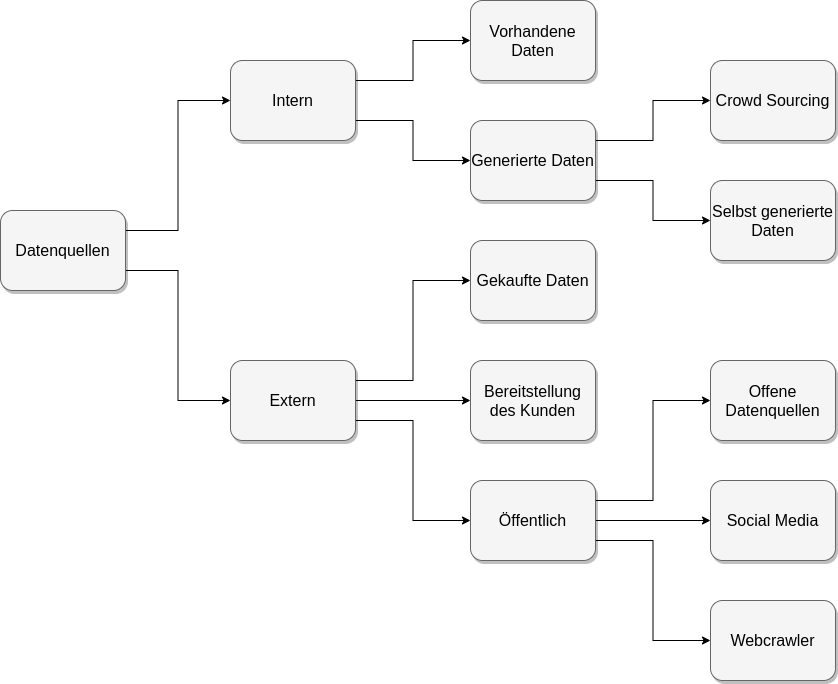
\includegraphics[width=0.7\textwidth]{datasources}
    \label{figure:datasources}
    \\
    \cite[Quelle: In Anlehnung an][Abb. 1]{hartmann2016capturing}
\end{figure}

Auf Basis von Abbildung \ref{figure:datasources} ist in der ersten Ebene eine Einteilung der Daten in interne und externe
Datenquellen möglich. Diese Unterteilung beschreibt die Herkunft der Daten.\footcite[Vgl.][Abb. 1]{hartmann2016capturing}
Interne Datenquellen stellen Daten zur Verfügung, die ausschließlich innerhalb einer Organisation zugänglich sind. Zu diesen
Datenquellen zählen folgend Daten der Mining Hardware, von \ac{ERP} Systemen und der Personalplanung. Bei den externen
Datenquellen gibt es eine dreiteilige Unterscheidung in gekaufte Daten, Daten, die durch einen Kunden bereitgestellt werden,
und öffentlich verfügbare Daten. Bei dieser Unterscheidung werden in Kapitel \ref{toc:externedatenquellen} primär die
öffentlichen Datenquellen betrachtet, da im Betrieb von Kryptomining Rechenzentren der Kundenfaktor erstmal ignoriert werden
kann. Zu diesen Datenquellen zählen öffentliche Blockexplorer, Mining Pools, Tauschbörsen, Wetter- und Klimadaten sowie
Daten aus Social Media Plattformen. Die Daten werden nach den folgenden Eigenschaften hin analysiert:
\begin{itemize}
    \item \textbf{Datenstruktur: }Daten können in strukturierte und unstrukturierte Daten unterteilt werden. Beispiele für
    strukturierte Daten sind Finanzdaten oder Sensordaten.\footcite[Vgl.][S. 27]{kimble2015big} Unstrukturierte Daten
    können Bilder, Texte oder Daten aus Social Media Plattformen sein.\footcite[Vgl.][S. 27]{kimble2015big}Diese Unterteilung
    hat Einfluss auf den \ac{ETL} Prozess, da Data Warehouses ausschließlich strukturierte Daten abspeichern
    können.\footcite[Vgl.][S.21]{niu2009cognition} Im Falle der Verwendung von unstrukturierten Daten müssen diese so angepasst
    werden, dass sie strukturiert werden.
    \item \textbf{Verfügbarkeit: }Mit diesem Parameter wird die Dauer von der Erhebung eines Datenpunktes bis hin zur
    Verfügbarkeit für Nutzer der Software gemessen. Gerade auf die Analyseprozesse kann dieser Parameter Auswirkungen
    haben, da dieser entscheidet, ob ein System benötigt wird, dass Echtzeitdaten verarbeiten muss oder beispielsweise nur
    Stapelverarbeitung betreibt. Die Ergebnisse aus dieser Kategorie werden in der Einschätzung der in Frage kommenden
    Analyseprozesse in Kapitel \ref{toc:analyseverfahrenbi} verwendet.
    \item \textbf{Konsistenz: }Diese Metrik sagt aus, ob die Daten, die durch die Quellsysteme zur Verfügung gestellt werden,
    frei von Widersprüchen sind. Falls Daten nicht widerspruchsfrei sind, kann dies zu Fehlern in den Analyseprozessen führen,
    die daher genau beobachtet werden müssen.\footcite[Vgl.][S. 561]{huh1990data} Da das Auswirkungen auf die Gestaltung
    der Analyseprozesse hat, muss diese Tatsache mit in Betracht gezogen werden.
\end{itemize}

\subsubsection{Interne Datenquellen} \label{toc:internedatenquellen}

In diesem Teil werden die internen Datenquellen und deren Daten klassifiziert, die für die Konzeption eines \ac{BI} Prozesses
in Betracht gezogen werden können.

\begin{itemize}
    \item \textbf{Mining Hardware / Überwachungssoftware: }
    Die technischen Parameter während des Betriebes werden durch die Mining Hardware generiert. Diese Parameter lassen
    Rückschlüsse auf die Effektivität der Hardware während des Mining Prozesses zu. Dazu zählen Daten, wie Hashrate, Temperatur,
    Hardwaredefekte und Stromverbrauch.\footcite[Vgl.][S. 12]{antminer2021manual} Diese Metriken sind über \acp{API} oder
    durch die \ac{SSH} Schnittstelle abfragbar.\footcite[Vgl.][]{awesomeminer2021api} Da die Konfiguration und Überwachung
    vieler einzelner Geräte einen zu hohen Aufwand und Zeitverbrauch für das Personal darstellt, wird Software eingesetzt,
    die in der Lage ist, eine große Anzahl von Mining Geräten zu überwachen und zu konfigurieren. Um dies zu erreichen, wird
    die \ac{API} oder \ac{SSH} Schnittstelle der Mining Hardware verwendet. Durch den Einsatz der Software können auch die
    Ausfallszeiten der Mining Hardware und der Stromverbrauch der Kühlung eines Rechenzentrums gemessen werden. Zusätzlich
    wird diese Software durch das Wartungspersonal verwendet, um defekte Geräte ausfindig zu machen und diese zu reparieren.
    Die Informationen zur Reparatur werden durch das Personal in das System eingetragen.
    \begin{itemize}
        \item Datenstruktur: Da es sich bei den Daten, welche die Mining Hardware generieren und die in der Überwachungssoftware
        gesammelt werden, letztendlich ausschließlich um Sensordaten handelt, sind die Daten aus dieser Quelle
        strukturiert.\footcite[Vgl.][S. 27]{kimble2015big}
        \item Verfügbarkeit: Die Verfügbarkeit der Daten in der Überwachungssoftware liegt bei circa fünf bis zehn Minuten,
        da diese Daten über regelmäßige Stapelverarbeitungsprozesse abgefragt werden.
        \item Konsistenz: Die Konsistenz ist gegeben. Alle diese Daten werden in relationalen Zeitreihen gespeichert. 
    \end{itemize}
    \item \textbf{ERP System: }Finanzielle \acp{KPI} werden meist in \ac{ERP} Systemen
    gespeichert.\footcite[Vgl.][Tabelle 3]{spathis2003usefulness} Diese Systeme werden dafür benutzt, die finanziellen \acp{KPI}
    eines Rechenzentrums zu erhalten. Diese Daten sind beispielsweise Anschaffungskosten, Kosten des Managements,
    Elektrizitätskosten und Personalkosten. Eine ausführliche Auflistung findet sich in
    Kapitel \ref{toc:kennzahlenundeinflussfaktoren}. In den folgenden Betrachtungen werden diese Daten in die Kategorien
    \ac{CapEx} und \ac{OpEx} aufgeteilt, da dies für die Prüfung der Hypothesen ausreichend ist. Durch die Schnittstellen
    der ERP Systeme sind diese Daten einheitlich abfragbar.
    \begin{itemize}
        \item Datenstruktur: Da es sich bei diesen Daten vorrangig um Finanzdaten handelt und diese durch die Schnittstelle
        des ERP Systems abgefragt werden, handelt es sich um strukturierte Daten.\footcite[Vgl.][S. 27]{kimble2015big}
        \item Verfügbarkeit: Sobald diese Daten in einem \ac{ERP} System eingetragen sind, sind diese auch direkt abfragbar.
        Daher bietet ein \ac{ERP} System Echtzeitdaten an.
        \item Konsistenz: Ausgehend von der Annahme, dass die eingehenden Daten korrekt sind, sind die Informationen aus
        einem \ac{ERP} System widerspruchsfrei und damit konsistent.
    \end{itemize}
    \item \textbf{Personalplanung: }Letztendlich sind die Planungssysteme für das Personal intern verfügbar. Diese
    beinhalten die Zahl der Angestellten, deren Gehälter und deren Arbeitszeiten. Zusätzlich zu den Arbeitszeiten sind die
    Schichtpläne der Rechenzentren in diesen Systemen verfügbar, worüber Schlussfolgerungen über die Personalbeschaffenheit
    vor Ort gemacht werden können. Diese Daten sind über standardisierte Schnittstellen abfragbar.
    \begin{itemize}
        \item Datenstruktur: Die Daten, die das Personalsystem zur Verfügung stellt, sind strukturiert und relational.
        \item Verfügbarkeit: Die Verfügbarkeit solcher Daten ist direkt und ohne Zeitverzögerung abfragbar, sobald diese in
        das System eingetragen sind.
        \item Konsistenz: Unter der Voraussetzung, dass alle eingegebenen Daten korrekt sind, sind alle Daten eines
        Personalmanagementsystems widerspruchsfrei.
    \end{itemize}
\end{itemize}

In der folgenden Tabelle sind die Klassifizierungen der einzelnen Datentypen gelistet, die sich aus den oben genannten Datenquellen
ergeben.

\begin{table}[H]
    \caption{Klassifizierung der internen Datenquellen}
    \label{tbl:klassifizierunginternedaten}
    \begin{tabularx}{\textwidth}[ht]{X||c|c|c}
        Datenquelle & Datenstruktur & Verfügbarkeit & Konsistenz  \\
        \hline\hline
        Mining Hardware / Überwachungssoftware & Strukturiert & 5-10 Minuten & Konsistent \\
        \hline
        ERP System & Strukturiert & \specialcell{Echtzeit innerhalb\\der Software} & Konsistent \\
        \hline
        Personalplanung & Strukturiert & \specialcell{Echtzeit innerhalb\\der Software} & Konsistent \\
    \end{tabularx}
\end{table}

\subsubsection{Externe Datenquellen} \label{toc:externedatenquellen}

Analog zur Klassifizierung der internen Daten in Kapitel \ref{toc:internedatenquellen}, werden im Folgenden die externen
Datenquellen klassifiziert. Die folgenden relevanten externen Datenquellen sind identifizierbar:

\begin{itemize}
    \item \textbf{Öffentliche Blockexplorer: }Blockexplorer sind Webseiten, die die Daten der Blockchain über Schnittstellen
    abrufbar machen. Beispiele für Daten, die direkt auf der Blockchain liegen, sind die Difficulty oder auch die Höhe der
    Transaktionsgebühren der noch nicht bestätigten
    Transaktionen.\footcite[Vgl.][]{bitcoin2021getdifficulty}\footcite[Vgl.][]{bitcoin2021getrawmempool} Zusätzlich werden
    Metriken angeboten, die auf Basis der Daten auf der Blockchain berechnet oder abgeschätzt werden können. Dazu gehören
    Daten wie beispielsweise die Schätzung der Netzwerkhashrate des Bitcoin
    Netzwerks.\footcite[Vgl.][]{blockchain2021total}\footcite[Vgl.][]{blockchain2021api} Zusätzlich können über solche
    Blockexplorer auch jegliche blockchainbezogenen Daten in ihrer vollen Historie bezogen werden. Eine andere Möglichkeit,
    die Daten der Blockchain zu erhalten, wäre der Betrieb einer eigenen Bitcoin Node. Da der Betrieb und die Wartung davon
    viel Fachwissen verlangt, ist die Abfrage der Daten durch einen öffentlichen Blockexplorer zu bevorzugen.
    \begin{itemize}
        \item Datenstruktur: Die Beschaffenheit der Daten, die von einem Blockexplorer geliefert werden, sind strukturiert.
        Dies liegt vor allem an der strikten Strukturiertheit der Blockchain.
        \item Verfügbarkeit: Die Verfügbarkeit unterscheidet sich je nach abgefragten Parametern. Daten, die direkt auf
        der Blockchain gespeichert sind, sind in Echtzeit abfragbar. Beispiele dafür ist die Difficulty oder Informationen
        über Transaktionen.
        
        Alle weiteren Daten, die auf Basis der Blockchaindaten errechnet werden, aber nicht direkt von dieser stammen, werden
        meist nur einmal am Tag veröffentlicht. Ein Beispiel ist die hochgerechnete Gesamthashrate des Bitcoin Netzwerks.
        \item Konsistenz: Da die Widerspruchsfreiheit der Daten einer der Gründe für die Einführung von Blockchains waren,
        können folglich die Daten eines Blockexplorers auch als widerspruchsfrei und damit konsistent angesehen werden. 
    \end{itemize}
    \item \textbf{Mining Pools: }Wie in Kapitel \ref{toc:miningundkonsensalgorithmen} bereits gezeigt, gibt es die
    Möglichkeit, durch Mining Pools am Mining teilzunehmen. Ein Mining Pool bietet die Möglichkeit der Risikoreduzierung
    während des Mining Prozesses. Dafür verlangt dieser Nutzungsgebühren, die unterschiedlich bemessen sein
    können.\footcite[Vgl.][S. 59ff]{bhaskar2015bitcoin} Diese Gebühren können direkt von einem Mining Pool abgefragt werden
    und damit in die finanzielle Gesamteinschätzung Einzug halten. Da der Besitzer der Mining Hardware anteilig
    zu der zur Verfügung gestellten Hashrate am Ertrag des Pools beteiligt wird, ist bei einem Mining Pool die ankommende
    Hashrate nachvollziehbar. Diese kann mit der Hashrate der Mining Hardware verglichen werden, um Aussagen über die
    Netzwerkverbindungen treffen zu können. Alle diese Daten sind standardisiert über eine \ac{API} erhältlich.
    \begin{itemize}
        \item Datenstruktur: Die Daten über die Hashrates sind vergleichbar zu Sensordaten. Aus diesem Grund liefert ein
        Mining Pool strukturierte Daten aus.\footcite[Vgl.][S. 27]{kimble2015big}
        \item Verfügbarkeit: Die Daten sind mit einer Verzögerung von 15-30 Minuten abfragbar.
        \item Konsistenz: Die Daten sind konsistent, da diese auf der Basis von Zeitreihen erhoben werden. Es können
        Unterschiede zur Hashrate der Mining Hardware gemessen werden. Diese sind allerdings keine Inkonsistenz, sondern
        geben Rückschlüsse auf die Verbindungsqualität zwischen Rechenzentrum und Mining Pool.
    \end{itemize}
    \item \textbf{Tauschbörsen: }Die Tauschbörsen werden verwendet, um die durch den Mining Prozess verdienten Bitcoins in
    Fiat Währungen umtauschen zu können. Dabei sind zwei Hauptfaktoren zu beachten. Das ist zum einen der momentane Tauschkurs
    zwischen \ac{BTC} und \ac{USD}. Zum anderen müssen die Handelsgebühren einer Tauschbörse noch zusätzlich in Betracht
    gezogen werden. Alle diese Werte unterscheiden sich von Börse zu Börse. Tauschbörsen haben umfangreiche und
    performante \acp{API}, um mit diesen sehr schnell handeln zu können.
    \begin{itemize}
        \item Datenstruktur: Tauschbörsen bieten strukturierte Daten an. Nur diese Form der Daten lässt eine sehr schnelle
        Bearbeitung und Analyse zu.\footcite[Vgl.][S. 27]{kimble2015big}
        \item Verfügbarkeit: Die Schnittstellen der Börse stellen Daten in Echtzeit bereit.
        \item Konsistenz: Die Daten der Tauschbörsen müssen konsistent sein, da sonst Probleme im Handel auftreten können.
    \end{itemize}
    \item \textbf{Wetter- und Klimadaten: }Betreiber von Kryptomining Rechenzentren sind durch die dynamische Anpassung der
    Kühlungsanlagen an die Außentemperatur in der Lage, Energiekosten einzusparen. Um dieses Einsparungspotential nutzen zu
    können, werden Schnittstellen benötigt, an denen aktuelle und historische Wetterdaten abfragbar sind. Ein Beispiel für
    eine umfassende Schnittstelle ist World Weather Online.\footcite[Vgl.][]{wwo2021api} Diese Schnittstelle verlangt ein Entgelt
    für die Nutzung, da die Bereitstellung von weltweiten Wetterdaten komplex ist.\footcite[Vgl.][]{wwo2021pricing} Gerade bei
    einem Neubau eines Rechenzentrums macht die Einbeziehung von Klimadaten Sinn, um den Stromverbrauch und die Dimensionierung
    der Kühlungsanlagen abschätzen zu können.
    \begin{itemize}
        \item Datenstruktur: Wetter- und Klimadaten werden strukturiert zur Verfügung gestellt, um eine gute Analyse ermöglichen
        zu können.
        \item Verfügbarkeit: Die Daten werden laut World Weather Online in Echtzeit zur Verfügung
        gestellt.\footcite[Vgl.][]{wwo2021api}
        \item Konsistenz: Die Konsistenz der Daten ist wichtig und innerhalb einer Plattform auch gegeben. Bei der Abfrage
        mehrerer Quellen für Wetterdaten kann es zu Inkonsistenzen kommen.
    \end{itemize}
    \item \textbf{Social Media: }Anfang des Jahres 2021 war beobachtbar, dass durch Social Media Plattformen der Bitcoin
    Wechselkurs stark beeinflusst wurde
    (Vgl. Abb. \ref{figure:btctweets}).\footcite[Vgl.][]{forbes2021musk}\footcite[Vgl.][S. 1f]{ante2021elon} Daher darf in
    einer Einschätzung der Wechselkurse der Einfluss von Social Media inzwischen nicht mehr ignoriert werden. In Social Media
    ist es durch die Analyse von beispielsweise Hashtags möglich, ein Stimmungsbild zu ermitteln. Auch können Äußerungen von
    reichweitenstarken Personen oder Gruppen, die kursbeeinflussend sind, schnell analysiert werden.
    \begin{itemize}
        \item Datenstruktur: Die Daten von Social Media Plattformen sind unstrukturiert.\footcite[Vgl.][S. 27]{kimble2015big}
        \item Verfügbarkeit: Die Verfügbarkeit von Daten über Web Scraping oder \acp{API} ist in Echtzeit gegeben.
        \item Konsistenz: Da an Social Media Plattformen grundsätzlich jeder Mensch teilnehmen kann, sind die Daten, die
        analysiert werden können, inkonsistent.
    \end{itemize}
\end{itemize}

\begin{figure}[H]
    \caption{Bitcoin Wechselkurs im Vergleich mit den Anzahl der Tweets mit Hashtag \#bitcoin pro Tag}
    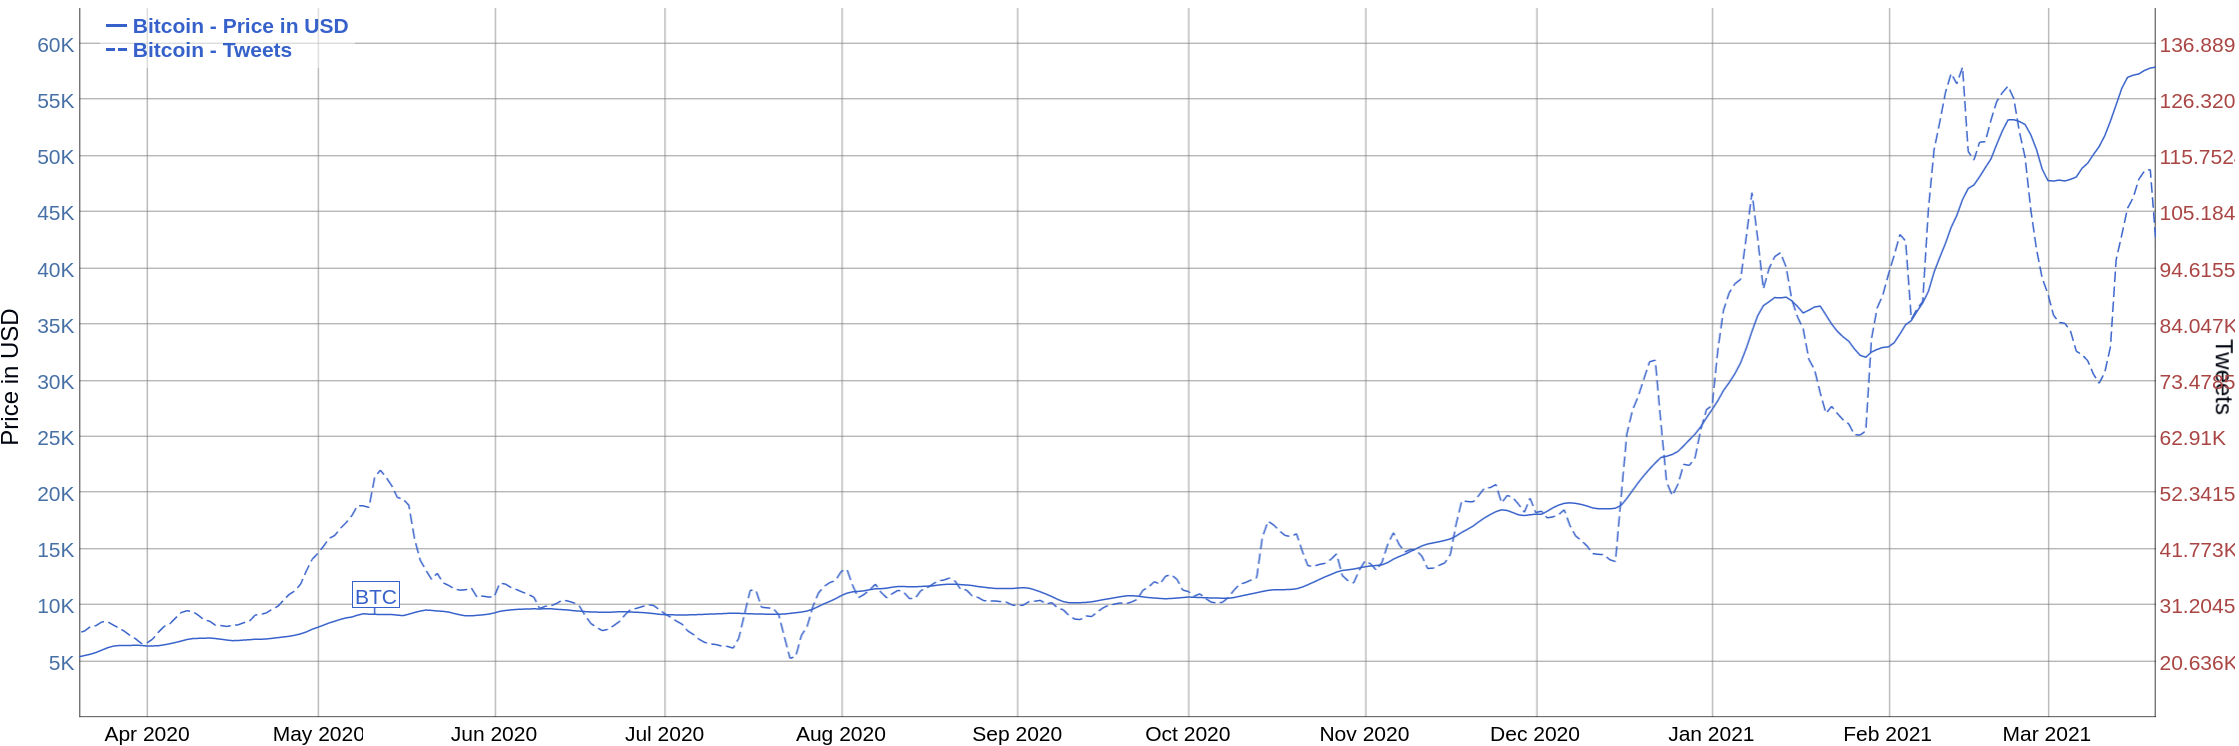
\includegraphics[width=\textwidth]{tweetsbitcoin}
    \label{figure:btctweets}
    \\
    \cite[Quelle: Vgl.][]{bitinfocharts2021bitcointweets}
\end{figure}

Zusammenfassend sind die erarbeiteten Klassifizierungen in Tabelle \ref{tbl:klassifizierungexternedaten} aufgelistet.

\begin{table}[H]
    \caption{Klassifizierung der externen Datenquellen}
    \label{tbl:klassifizierungexternedaten}
    \begin{tabularx}{\textwidth}[ht]{X||c|c|c}
        Datenquelle & Datenstruktur & Verfügbarkeit & Konsistenz  \\
        \hline\hline
        Öffentliche Blockexplorer (Daten der Blockchain) & Strukturiert & Echtzeit & Konsistent \\
        \hline
        Öffentliche Blockexplorer (Metriken basierend auf Blockchaindaten) & Strukturiert & 24 Stunden & Konsistent \\
        \hline
        Mining Pools & Strukturiert  & 15-30 Minuten & Konsistent \\
        \hline
        Tauschbörsen & Strukturiert & Echtzeit & \specialcell{Konsistent innerhalb\\jeder Tauschbörse} \\
        \hline
        Wetter- und Klimadaten & Strukturiert & Echtzeit & \specialcell{Konsistent innerhalb\\jedes Wetterdienstes} \\
        \hline
        Social Media & Unstrukturiert & Echtzeit & Inkonsistent \\
    \end{tabularx}
\end{table}

\subsection{Prüfung der Teilhypothesen} \label{toc:pruefungderteilhypothesen}

Basierend auf der Klassifizierung der möglichen Datenquellen und deren verfügbaren Informationen wird in diesem Teil die Prüfung
der Teilhypothesen vorgenommen. Dazu wird für jede einzelne Teilhypothese definiert, welche \acp{KPI} relevant sind, um diese
zu evaluieren und final zu verifizieren. Dafür werden die \acp{KPI} aus den Kapiteln \ref{toc:technologie} und
\ref{toc:miningrechenzentren} verwendet. Zusätzlich werden die Ergebnisse über die verfügbaren Datenquellen aus Kapitel
\ref{toc:klassifizierungderdaten} mit einbezogen, um Datenflüsse für eine \ac{BI} Implementierung zu identifizieren. Diese
werden für die Beantwortung der Hypothese verwendet. Abbildung \ref{figure:ht01dataflow} bis \ref{figure:ht04dataflow} machen
es möglich zu prüfen, welche Daten benötigt werden, ob diese für \ac{BI} verwendbar sind und ob diese zur Verfügung stehen.
In Kapitel \ref{toc:analyseverfahrenbi} wird besprochen, welche Analyseverfahren für die Daten benötigt werden, um letztendlich
die Teilhypothesen evaluieren und prüfen zu können. Dabei wird auch auf die verschiedenen Arten von \ac{BI} - deskriptive
(descriptive), vorhersagende (predictive) und präskriptive (prescriptive) Business Intelligence - und deren mögliche
Limitationen im Bereich Kryptomining eingegangen.\footcite[Vgl.][S. 96]{bihani2014comparative}

\subsubsection{Identifikation der Key Performance Indikatoren der Hypothesen} \label{toc:identifikationkpi}

Wie in der Einleitung zu diesem Kapitel bereits geschrieben, werden in diesem Teil die Datenquellen und die logischen Datenflüsse
identifiziert. Dazu werden alle vier Teilhypothesen getrennt betrachtet und jeweils ein zugeschnittener Abhängigkeitsbaum der
Informationen und \acp{KPI} definiert. Diese finden sich zusammengefasst in den jeweiligen Abbildungen, die zu den Teilhypothesen
gehören. Generell wird zwischen finanziellen, technischen und personellen \acp{KPI} unterschieden. Dahinter werden die
dementsprechenden Datenquellen aus Kapitel \ref{toc:klassifizierungderdaten} genannt, die von Relevanz sind. In der letzten Ebene
werden die einzelnen Datentypen, die benötigt werden, benannt. Im Folgenden wird diese Analyse für alle vier Teilhypothesen
durchgeführt:

\begin{itemize}
    \item \textbf{\ac{HT0.1}: }Diese Teilhypothese prüft einen möglichen Einfluss von \ac{BI} auf Entscheidungsprozesses des
    Managements in Bezug auf den Neu- und Ausbau von Kryptomining Rechenzentren. Eine solche Entscheidungsunterstützung benötigt
    eine Vielzahl an Daten, da ein Neu- oder Ausbau eine komplexe strategische Entscheidung darstellt. Aus diesem Grund werden alle
    drei Formen von \acp{KPI} - personelle, technische und finanzielle - benötigt.
    
    Diese strategische Entscheidung basiert auf Faktoren hinsichtlich des Ortes, der Auswahl der Hardware und der
    Tauschgeschäfte von Bitcoin in Fiat Währungen, um die Rechenzentren zu finanzieren. Die Auswahl des Ortes beeinflusst
    jegliche Formen der bereits beschriebenen \acp{KPI} und beruht damit auf Daten, wie Personalgehälter, \ac{CapEx}, \ac{OpEx}
    und Energieverbrauch der Mining Hardware. Die Auswahl der Hardware wiederum wird durch Faktoren, wie Hashrate, Ausfallszeiten
    (Stabilität der Hardware) und dem Energieverbrauch, bestimmt. Die Tauschgeschäfte werden durch die Daten, die Tauschbörsen
    anbieten, maßgeblich bestimmt.
    
    Nach Tabelle \ref{tbl:klassifizierunginternedaten} und \ref{tbl:klassifizierungexternedaten} sind alle diese Daten
    strukturiert und konsistent. Daher eignen sich diese Datenquellen ohne weiteres für die Verwendung in \ac{BI} Prozessen.
    Der \ac{ETL} Vorgang für die einzelnen Datenquellen lässt sich durch die genannten Grundeigenschaften der Daten problemlos
    aufbauen, damit die Daten durch ein Data Warehouse für die weiteren Teilprozesse verfügbar gemacht werden. Die Verfügbarkeit
    der verwendeten Daten unterscheidet sich je nach Datentyp. Bei Tauschbörsen sind die Daten direkt in Echtzeit abfragbar.
    Im Gegensatz dazu gibt es bei den technischen \acp{KPI} eine Verzögerung von circa fünf bis zehn Minuten.  Systeme wie
    \ac{ERP} und Personalerfassung liefern Daten in Echtzeit, sobald diese dem System vorliegen. Da strategische Entscheidungen,
    wie der Neu- oder Ausbau von Mining Rechenzentren, allerdings langwierige Entscheidung sind, limitiert die Verfügbarkeit
    die Hypothese nicht.

    Anhand der nun verfügbaren Daten wird im folgenden Kapitel evaluiert, ob es möglich ist, diese Daten in einer Art und Weise zu
    analysieren, sodass am Ende daraus zusätzliches Wissen generiert werden kann und damit diese Daten zur Entscheidungsunterstützung
    verwendet werden können.

    \begin{figure}[H]
        \caption{Relevante KPIs, Datenquellen und Datentypen für Teilhypothese 1}
        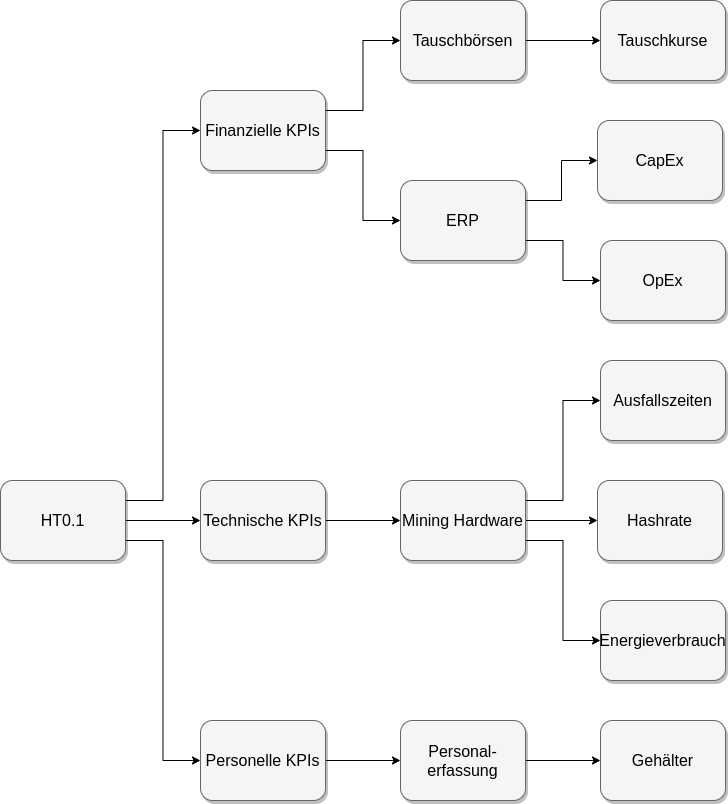
\includegraphics[width=0.55\textwidth]{ht01dataflow}
        \label{figure:ht01dataflow}
    \end{figure}

    \item \textbf{\ac{HT0.2}: }Diese Teilhypothese beschäftigt sich mit dem Einfluss von \ac{BI} auf die Effektivität der
    Mining Hardware. Da diese Hypothese ausschließlich technischer Natur ist, werden dafür nur technische \acp{KPI}, wie
    Stromverbrauch, Hashrate, Ausfallszeiten und Hardwaredefekte, benötigt. Diese Daten stammen ausschließlich aus dem
    Überwachungssystem der Mining Hardware. Nach Tabelle \ref{tbl:klassifizierunginternedaten} sind diese Daten sowohl
    konsistent als auch strukturiert, wodurch sich diese Daten für ein \ac{BI} Konzept eignen. Die \ac{ETL} Pipelines sind
    für diese Art von Daten einfach zu errichten. Die verzögerte Verfügbarkeit der Daten (fünf bis zehn Minuten) stellt keine
    Probleme für die Hypothese dar, da diese nicht zwingend auf Echtzeitdaten angewiesen ist. Gerade bei der Messung von
    Effektivitäten im Mining Prozess braucht man längere Zeitfenster von mehreren Tagen, um belastbare Aussagen zu erhalten.
    Anhand der Datenquellen können Faktoren berechnet werden, die Einfluss auf die Effektivität des Mining Prozesses haben.
    Dazu gehören die Hashrate der eigenen Mining Hardware, deren Energieeffizienz ("`Reference power effiency"',
    $\frac{J}{TH}$) und die Messung der Uptime und der Gerätedefekte, die beispielsweise durch bessere Firmwares optimiert
    werden können.

    \begin{figure}[H]
        \caption{Relevante KPIs, Datenquellen und Datentypen für Teilhypothese 2}
        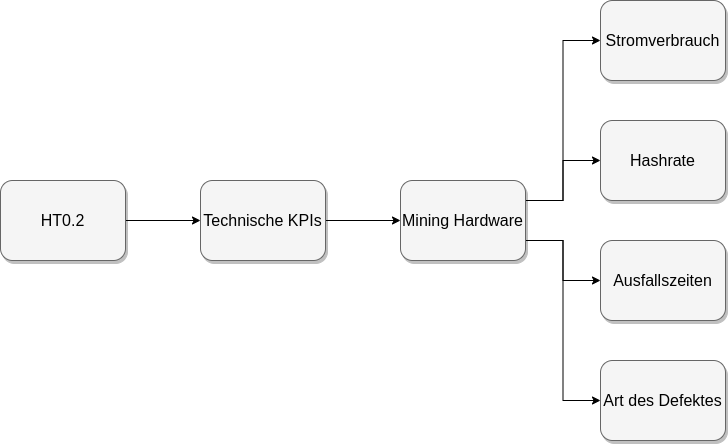
\includegraphics[width=0.55\textwidth]{ht02dataflow}
        \label{figure:ht02dataflow}
    \end{figure}

    \item \textbf{\ac{HT0.3}: }Die dritte Teilhypothese beschreibt die Verbesserung des Cashflows eines Kryptomining
    Rechenzentrums durch die Anwendung von \ac{BI}. Um die Hypothese zu prüfen, werden technische und finanzielle \acp{KPI}
    benötigt. Unter den technischen \acp{KPI} finden sich Parameter, wie Hashrate und Informationen aus öffentlichen
    Blockexplorern, wie beispielsweise die Difficulty und die Hochrechnung der Netzwerkhashrate. Durch diese Informationen ist
    der theoretische Mining Ertrag durch die Hardware prognostizierbar. Die finanziellen \acp{KPI} teilen sich in Tauschbörsen,
    \ac{ERP} Systeme und Mining Pools auf. Die Tauschbörsen liefern Daten zu ihren Handelsgebühren und den Tauschkursen von
    \ac{BTC}. Diese werden benötigt, um die erhaltenen Bitcoins unter möglichst guten Bedingungen in Fiat Währungen tauschen
    zu können. Eine weitere finanzielle Datenquelle sind \ac{ERP} Systeme, die einen vollständigen finanziellen Überblick
    aller \ac{CapEx} und \ac{OpEx} Posten bieten. Letztendlich werden noch Informationen des Mining Pools verwendet (Gebühren
    und Ertrag), um einen Pool mit möglichst hoher Auszahlung zu identifizieren und zu verwenden. Anhand von Tabelle
    \ref{tbl:klassifizierunginternedaten} und \ref{tbl:klassifizierungexternedaten} stellen alle Quellsysteme bei richtiger
    Verwendung strukturierte und in sich konsistente Daten bereit. Wie bereits in den Punkten \ac{HT0.1} und \ac{HT0.2}
    festgestellt, ist daher eine Integration in einen \ac{BI} Prozess möglich. Nicht alle benötigten Daten werden in Echtzeit
    bereitstellt. Dazu zählen \acp{KPI}, wie Mining Pool Gebühren und Erträge (15-30 Minuten), Netzwerkhashrate (24 Stunden)
    und Hashrate der Mining Hardware (fünf bis zehn Minuten). Da der Cashflow eine finanzielle Größe ist, die nur auf großen
    Zeitspannen (> 1 Tag) sinnvoll errechnet werden kann, stellt diese Verzögerung kein Problem für die Verwendung der Daten
    innerhalb eines \ac{BI} Prozesses dar.

    \begin{figure}[H]
        \caption{Relevante KPIs, Datenquellen und Datentypen für Teilhypothese 3}
        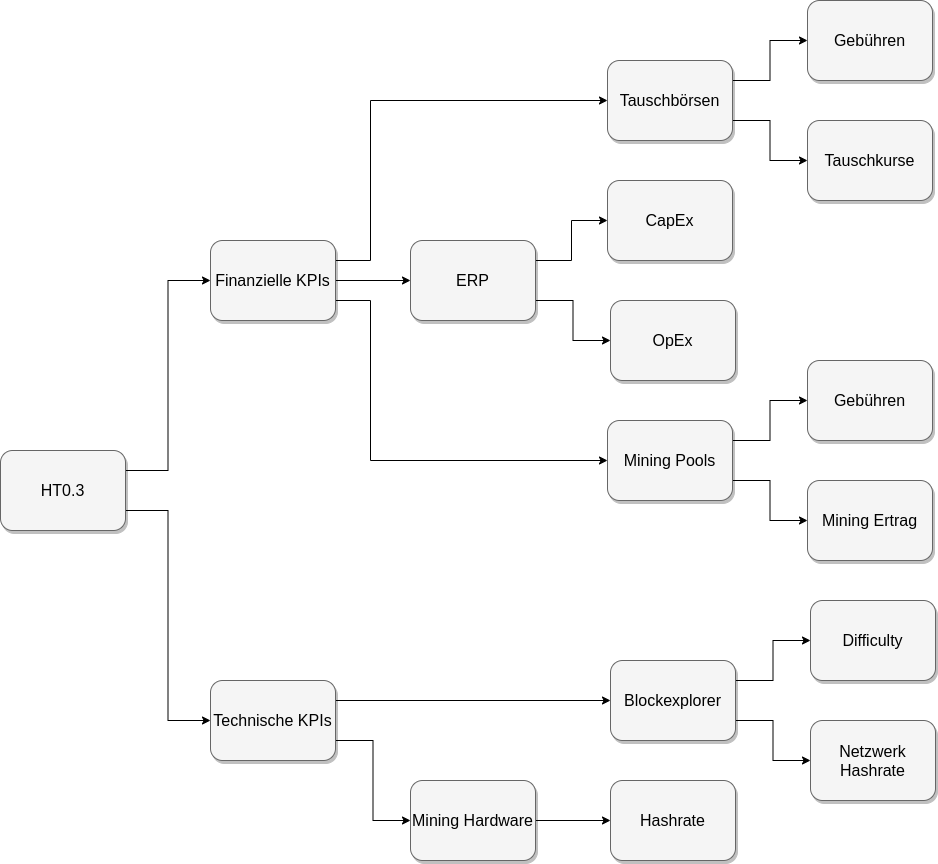
\includegraphics[width=0.7\textwidth]{ht03dataflow}
        \label{figure:ht03dataflow}
    \end{figure}

    \item \textbf{\ac{HT0.4}: }Die letzte Teilhypothese ist im Bereich der Personalplanung anzusiedeln und sagt aus, dass
    diese durch die Anwendung eines \ac{BI} Prozesses optimiert werden kann. Zur Beantwortung dieser Hypothese sind sowohl
    die technischen \acp{KPI} als auch die personellen \acp{KPI} von Bedeutung. Zu den technischen Indikatoren zählen Daten,
    wie die Ausfallzeiten und Informationen über die Art des Hardwaredefekts. Zu den personellen \acp{KPI} zählen wiederum Daten,
    wie Schichtpläne und Ausbildungen des Personals. Durch die Bereitstellung dieser Datenquellen ist es möglich, die
    durchschnittliche Dauer eines Reparaturvorgangs zu errechnen und anhand dessen die Personaldecke vor Ort realistisch
    einschätzen zu können. Nach Tabelle \ref{tbl:klassifizierunginternedaten} sind alle Daten konsistent und strukturiert,
    wodurch eine Verwendung dieser Daten in einem \ac{BI} möglich ist. Die \ac{ETL} Pipelines sind ohne weiteres realisierbar.
    Die technischen \acp{KPI} sind allerdings nur mit einer Verzögerung von fünf bis zehn Minuten zugänglich. Dies stellt jedoch
    für die Realisierbarkeit dieser Hypothese kein Problem dar, da andere Daten, wie beispielsweise neue Schichtpläne, nur einmal
    pro Monat aktualisiert werden und daher die Errechnung relevanter Ergebnisse nicht durch diese Verzögerung signifikant
    beeinflusst wird.

    \begin{figure}[H]
        \caption{Relevante KPIs, Datenquellen und Datentypen für Teilhypothese 4}
        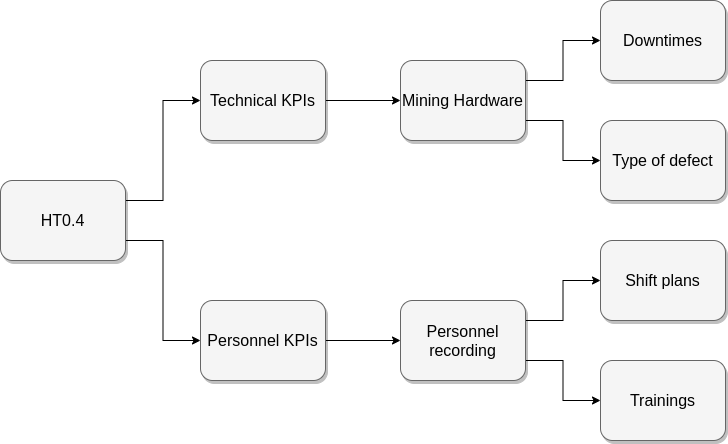
\includegraphics[width=0.55\textwidth]{ht04dataflow}
        \label{figure:ht04dataflow}
    \end{figure}
\end{itemize}

\subsubsection{Erforderliche Analyseverfahren innerhalb des Business Intelligence Prozesses} \label{toc:analyseverfahrenbi}

Um nun die Hypothesen final prüfen zu können, wird in diesem Kapitel geklärt, ob bereits etablierte Analyseprozesse dazu
ausreichen, die relevanten Daten für eine Hypothese so nutzbar zu machen, dass daraus Wissen generiert werden kann. Um dies
zu erreichen, werden die vorhandenen Analyseverfahren aus der Veröffentlichung von Bihani und Patil dem deskriptiven,
vorhersagenden oder präskriptiven Paradigma von \ac{BI} zugeordnet und analysiert, ob damit die einzelnen Teilhypothesen
beantwortet werden können:\footcite[Vgl.][S. 97ff]{bihani2014comparative}\footcite[Vgl.][Abb. 2]{bihani2014comparative}

\begin{itemize}
    \item \textbf{Deskriptive Analyse: }Diese Punkt beschreibt die Analyse der vergangenen und bereits erhobenen
    Daten. Die folgenden Analyseverfahren können für den deskriptiven Ansatz verwendet
    werden:\footcite[Vgl.][S. 97ff]{bihani2014comparative}
    \begin{itemize}
        \item \textbf{Faktorenanalyse: }Durch diese Form der Analyse werden unterliegende Strukturen in den Daten
        herausgefunden.\footcite[Vgl.][S. 97f]{bihani2014comparative} Dazu werden große multidimensionale Datensätze verwendet
        und diese zu kleineren Datensätze reduziert, die eine Aussagekraft haben. Diese Datensätze beinhalten dadurch
        grundlegende Faktoren, die die gemessenen großen Datensätze erklären
        können.\footcite[Vgl.][S. 97f]{bihani2014comparative} Solche Analysen sind unter anderem mittels \ac{OLAP} Systemen
        realisierbar. Für die Beantwortung der Teilhypothesen kann diese Form der Analyse verwendet werden. Es existieren
        in einem Data Warehouse, das die in Kapitel \ref{toc:klassifizierungderdaten} aufgeführten Daten beinhaltet, große
        Datensätze, wie beispielsweise die Hashrate der Mining Hardware oder auch Tauschkurse von \ac{BTC} in \ac{USD}. Auch
        ein Vergleich dieser Größen ist sinnvoll, wie beispielsweise von \ac{OpEx} und der Gesamthashrate eines Rechenzentrums.
        Aus diesen Gründen können die Faktorenanalyse und \ac{OLAP} Systeme für alle Teilhypothesen Sinn machen.
        \item \textbf{Clusteranalyse: }Dies ist ein Algorithmus der Ähnlichkeiten in Datensätzen identifizieren
        kann.\footcite[Vgl.][S. 98]{bihani2014comparative} Dadurch können Teilmengen der Datensätze als zusammenhängend
        klassifiziert werden. Unter den Überbegriff Clusteranalyse fallen viele Algorithmen, die aus dem Bereich "`Data Mining"'
        bekannt sind. Dazu zählt der "`K-Means-Algorithmus"' oder "`Nearest Neighbor"'.\footcite[Vgl.][S. 98]{bihani2014comparative}
        Das Ziel, große Datensätze durch Clustering Algorithmen zu unterteilen, bietet auch die Möglichkeit, die Strukturierung
        der Daten weiter erforschen zu können. Gerade bei den technischen \acp{KPI} ist daher diese Form der Analyse passend.
        Damit ist die Clusteranalyse für alle Teilhypothesen relevant und kann bei der Analyse von Hilfe sein. 
        \item \textbf{Diskriminanzfunktionsanalyse: }Die Analyse kann die Abweichung zweier gemessener Gruppen von Werten
        messen und dadurch bestimmen, ob eine Trennung existiert und wie stark diese
        ist.\footcite[Vgl.][S. 98]{bihani2014comparative} Die Anwendung dieser Analyse liegt klassischerweise im Verständnis
        von demographischen Faktoren beim Kauf von Produkten.\footcite[Vgl.][S. 98]{bihani2014comparative} Interessant ist diese
        Form der Analyse für die Interpretation der identischen \acp{KPI} aus verschiedenen Rechenzentren. Gerade die Analyse von
        Unterschieden von Daten zwischen Rechenzentren ermöglicht die Generierung von neuem Wissen und ist somit im Bereich
        \ac{BI} von unmittelbarer Relevanz. Die Anwendung der Diskriminanzfunktionsanalyse ist daher für alle Teilhypothesen
        sinnvoll, sobald mehr als ein Rechenzentrum betrachtet wird.
        \item \textbf{Strukturgleichungsmodell: }Dabei werden Abhängigkeiten zwischen Variablen gebildet und mittels linearen
        Gleichungssystemen geprüft, ob diese Beziehung tatsächlich existiert.\footcite[Vgl.][S. 98f]{bihani2014comparative} Als
        Ergebnis wird die Abhängigkeit bzw. Unabhängigkeit von dem vorgegebenen Modell
        festgestellt.\footcite[Vgl.][S. 98f]{bihani2014comparative}
        Gerade um mögliche Abhängigkeiten zwischen den einzelnen \acp{KPI} festzustellen, kann diese Form der Analyse verwendet
        werden. Ein einfaches Beispiel ist die Abhängigkeit von der Hashrate zum Ertrag durch den Mining Pool. Aufgrund dessen
        findet das Strukturgleichungsmodell auch bei den vorliegenden Teilhypothesen sinnvolle Anwendung.
    \end{itemize}
    Zusammenfassend ist feststellbar, dass es eine Vielzahl von verschiedenen Möglichkeiten gibt, die vorliegenden Daten zu
    analysieren und dadurch Wissen für die Stakeholder generieren zu können. Mit Hilfe der vorliegenden Analyseformen ist
    ein deskriptiver \ac{BI} Prozess mit den Teilhypothesen durchführbar.

    \item \textbf{Vorhersagende Analyse: }Bei diesem Paradigma werden Modelle zur Vorhersage mittels verschiedener Werkzeuge
    gebildet. Viele dieser Werkzeuge kommen aus dem Bereich der Statistik und des maschinellen
    Lernens.\footcite[Vgl.][Abb. 1]{bihani2014comparative} Folgende Formen der Analyse kommen zusätzlich zu den bereits
    genannten Formen hinzu:
    \begin{itemize}
        \item \textbf{Regressionsanalyse: }Bei dieser Form der Analyse wird die Abhängigkeit einer Variable von einer oder
        mehreren Variablen geprüft.\footcite[Vgl.][S. 97f]{bihani2014comparative} Dabei gibt es mehrere Formen, wie die lineare
        oder die logistische Regression verwendet werden kann. Diese Analyse kann bei der Prognose der Profitabilität
        oder von Marktanteilen sehr gut verwendet werden.\footcite[Vgl.][S. 99]{bihani2014comparative} Aus diesem Grund kann
        diese auch für die zu prüfenden Teilhypothesen von Relevanz sein. Eine Anwendung der
        Regressionsanalyse ist die Prognose des Wertes von Bitcoins.\footcite[Vgl.][S. 19]{ibrahim2020bitcoin} Prinzipiell
        ist eine Vorhersage mit Hilfe dieser Mechanismen gut möglich. Ende 2020 sind Faktoren, wie Social Media dazugekommen,
        die diese Form der Analyse deutlich erschweren.\footcite[Vgl.][]{forbes2021musk} Demzufolge kann die Regressionsanalyse eine
        Methodik sein, um Kurse vorhersagen zu können, muss allerdings um weitere Analysemodelle erweitert werden, um ein gutes
        Gesamtbild zu erhalten. 
        \item \textbf{Stochastische Analyse: }Es ist möglich Vorhersagemodelle auf Basis von stochastischen Modellen zu
        simulieren. Ein bekanntes Beispiel für eine stochastische Analyse ist die "`Monte-Carlo-Simulation"'. Sie kann
        beispielsweise verwendet werden, um Preisentwicklungen und Entwicklungen der Gesamthashrate von Bitcoin für die Zukunft
        einschätzen zu
        können.\footcite[Vgl.][S. 28]{cocco2016modeling}\footcite[Vgl.][]{appendix:mcszenarien}\footcite[Vgl.][]{appendix:mcpreis}\footcite[Vgl.][]{appendix:mchashrate}
        Auch bei dieser Form der Simulation, die am 06.11.2020 angefertigt wurde ist feststellbar, dass diese die Entwicklungen
        des Bitcoin Kurses Anfang 2021 nicht vorhersagen konnte.\footcite[Vgl.][]{appendix:btcusd} Daher ist dieses Analysemodell für sich nicht direkt aussagekräftig,
        sondern muss durch weitere Modellierungen unterstützt werden.
    \end{itemize}

    Letztendlich kann festgehalten werden, dass der Bitcoin Preis nur bedingt vorhergesagt werden kann, da einige Einflussfaktoren, wie
    beispielsweise Social Media, nicht vorhergesagt werden können und sich mathematischen Möglichkeiten der Analyse weitestgehend entziehen.\footcite[Vgl.][]{forbes2021musk}\footcite[Vgl.][S. 325]{badertscher2017bitcoin}
    Generell ist dies allerdings kein ausschließliches Problem, das bei Bitcoin auftritt. Bei den klassischen Märkten ist das gleiche
    Problem bemerkbar. Aufgrund der hohen Volatilität des Bitcoin Kurses ist es in diesem Fall jedoch auffälliger.
    Andere \acp{KPI}, wie beispielsweise \ac{OpEx} Kosten oder technische \acp{KPI}, sind im Gegensatz dazu prognostizierbar, da diese
    wenig bis keine Schwankungen unterliegen und somit die Ergebnisse der deskriptiven Analyse unter diesem Paradigma weiterhin
    verwendet werden können. 
    Demnach ist feststellbar, dass \ac{HT0.2} und \ac{HT0.4} für Vorhersagemodelle geeignet sind, da diese ausschließlich \acp{KPI} verwendet,
    die in ausreichender Qualität simuliert werden können. Bei \ac{HT0.1} und \ac{HT0.3} können auch vorhersagende Modelle angewendet werden,
    wobei eine Limitation durch die Vorhersage des Bitcoin Kurses festgestellt werden kann. Dies kann durch eine geeignete Kombination der
    Analysemodelle verbessert werden. Falls es möglich ist, die unstrukturierten und inkonsistenten Daten aus Social Media Plattformen passend zu analysieren,
    sollten diese in die Vorhersagemodellierungen integriert werden. Um einen möglichst guten Eindruck des \ac{BTC} Kurses zu erhalten,
    ist es wichtig mit Echtzeitverarbeitung dieser Daten zu arbeiten.
    \item \textbf{Präskriptive Analyse: }Diese ist die höchste Stufe, die mit Hilfe von \ac{BI} Prozessen erreichbar ist. Dabei werden
    nicht nur Entscheidungshilfen dem Management zur Verfügung gestellt sondern es werden direkt Entscheidungen dem Management durch
    das System empfohlen. Die Analyse der Hypothese läuft ähnlich zu dem Punkt der Vorhersagemodelle, da diese Stufe von \ac{BI} auch
    auf diesen Modellen beruht. Demgemäß ist das Ergebnis dieser Analyse identisch mit der vorherigen und \ac{HT0.2} und \ac{HT0.4} sind in dieser 
    Stufe realisierbar. Wie bei dem vorherigen Punkt bereits aufgezeigt, haben die beiden anderen Hypothesen Limitationen, die aus
    der schlechten Vorhersagbarkeit des Bitcoin Kurses stammen. Eine Möglichkeit, dass die beiden Teilhypothesen doch für die
    präskriptive Analyse geeignet sind, wäre die Errechnung verschiedener Szenarien des Bitcoin Kurses und damit die Errechnung
    verschiedener Mining Erträge. Solche Vorhersagemodelle existieren innerbetrieblich bereits durch die Monte-Carlo-Simulation der Hashrate
    und des Bitcoin Kurses.\footcite[Vgl.][]{appendix:mcpreis}\footcite[Vgl.][]{appendix:mchashrate}
    Da die Antwort auf die Umsetzbarkeit eines solchen Systems nur schwer im Zuge dieser Argumenation gegeben werden kann, wird
    dies in der Fallstudie in Kapitel \ref{toc:planungeinesbiprozessesfuereinminingrechenzentrum} genauer betrachtet.
\end{itemize}

Außerhalb dieser Auflistung existieren noch zusätzliche Analyseformen, wie beispielsweise die Verbundsanalyse.\footcite[Vgl.][S. 97]{bihani2014comparative}
Diese findet beispielsweise bei Analyse des Kaufverhaltens von Kunden Anwendung. Aufgrund der nicht gefundenen Relevanz für den Anwendungsfall von Kryptomining
Rechenzentren wird diese Form nicht weiter in Betracht gezogen.

In Tabelle \ref{tbl:hypothesenanalyse} sind die Ergebnisse der vorhergehenden Analyse zusammenfassend visualisiert.

\begin{table}[H]
    \caption{Mögliche Analyseformen der Hypothesen}
    \label{tbl:hypothesenanalyse}
    \begin{tabularx}{\textwidth}[ht]{X||c|c|c|c}
        & \ac{HT0.1} & \ac{HT0.2} & \ac{HT0.3} & \ac{HT0.4}  \\
        \hline\hline
        Deskriptive Analyse & \checkmark & \checkmark & \checkmark & \checkmark \\
        \hline
        Vorhersagende Analyse & (\checkmark) & \checkmark & (\checkmark) & \checkmark \\
        \hline
        Präskriptive Analyse & (\checkmark) & \checkmark & (\checkmark) & \checkmark \\
    \end{tabularx}
    \begin{tablenotes}
        \item \hspace{1mm}\checkmark\hspace{10mm} Durchführbar
        \item (\checkmark)\hspace{8.5mm} Unter den beschriebenen Limitationen durchführbar
    \end{tablenotes}
\end{table}

Mit Abschluss dieses Kapitels ist geklärt, ob die Einführung eines \ac{BI} Prozesses für die jeweiligen Teilhypothesen möglich ist.
Im nächsten Kapitel werden schlussendlich die Ergebnisse der vier Teilhypothesen verwendet, um eine erste Aussage über die Haupthypothese
zu erhalten und damit die Forschungslücke, die diese Arbeit schließen soll, erstmalig zu beantworten.

\subsection{Zusammenfassende Betrachtung} \label{toc:zusammenfassendebetrachtung}

Nachdem in Kapitel \ref{toc:analyseverfahrenbi} die Prüfung der einzelnen Teilhypothesen vorgenommen wurde,
wird in diesem Teil dieses Wissen verwendet, um eine Aussage über die Haupthypothese zu erhalten.

Es existieren vier Stufen, die bei der Analyse von Daten erreicht werden können. Diese Stufen finden sich in Abbildung
\ref{figure:levelofanalysis}. Es wird folgend die Relevanz der Haupthypothese in den einzelnen Stufen evaluiert
und anhand dessen die Aussagen der Teilhypothesen auf die Haupthypothese projiziert. Die Stufen teilen sich
folgendermaßen auf:\footcite[Vgl.][Abb. 2]{bihani2014comparative}

\begin{figure}[H]
    \caption{Stufen der Datenanalyse}
    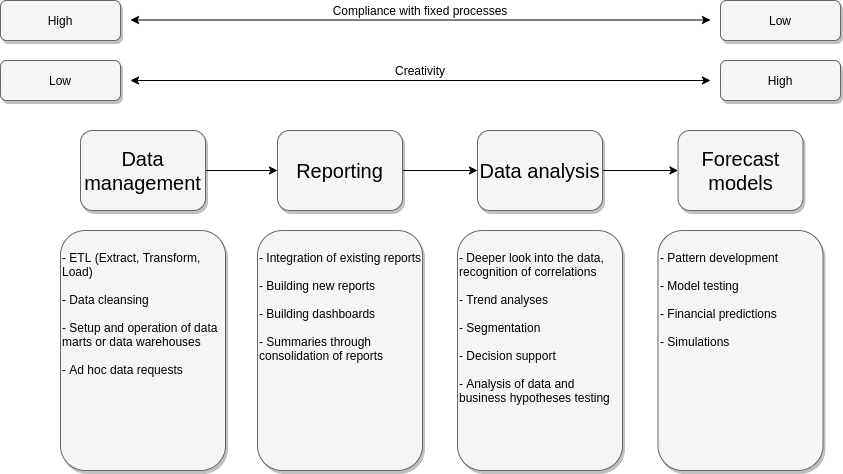
\includegraphics[width=0.8\textwidth]{levelofanalytics}
    \label{figure:levelofanalysis}
    \\
    \cite[Quelle: In Anlehnung an][Abb. 2]{bihani2014comparative}
\end{figure}

\begin{itemize}
    \item \textbf{Management der Daten: }Das Management der verschiedenen Daten ist ohne weiteres möglich. Alle relevanten
    Daten sind verfügbar und können in ein Data Warehouse eingespeist werden. Diese Analyse findet sich in Kapitel
    \ref{toc:internedatenquellen} und deren Zusammenfassungen in Tabelle \ref{tbl:klassifizierunginternedaten} und
    \ref{tbl:klassifizierungexternedaten}. Das Management der Daten ist auch für die Haupthypothese von unmittelbarer
    Wichtigkeit, da dies die Grundlagen für die Optimierung von Kryptomining Rechenzentren legt. Da bei allen Teilhypothesen
    das Management der Daten möglich ist, ist es das auch für die Haupthypothese. Es ist feststellbar, dass die erste
    Stufe ohne Probleme erreichbar ist.
    \item \textbf{Berichtswesen: }Die zweite Stufe der Verwendung von Daten ist die Errichtung eines Berichtwesens. Ein Berichtswesen
    verwendet die existierenden Daten der Vergangenheit, um für die Stakeholder des \ac{BI} Prozesses passende Berichte zu generieren.
    In diesem Fall sind dies Berichte, die die Teilhypothesen abdecken und damit personeller, technischer oder finanzieller
    Natur sind. Da diese
    Stufe deskriptiv ist, ist auch dies nach Tabelle \ref{tbl:hypothesenanalyse} für alle vier Teilhypothesen
    möglich. Daher ist möglich, das Berichtswesen für die Aussagen der Haupthypothese anzuwenden. Gerade diese Stufe ist für
    die Erreichung der zentralen Aussage der Haupthypothese ("`finanzielle Optimierung"') zentral, weil dies die Grundlage
    für die Optimierung eines Kryptomining Rechenzentrums legt.
    \item \textbf{Analyse der Daten: }Im dritten Schritt werden die Daten tiefer analysiert, um mehr Zusammenhänge zwischen den
    Daten feststellen zu können und damit mehr Wissen generieren zu können, was letztendlich für die Optimierung von Rechenzentren
    weiterhin verwendet werden kann. Daher ist auch die Haupthypothese in dieser Stufe anzutreffen. Dabei werden die bereits
    vorhandenen Daten verwendet, um Aussagen und Entscheidungshilfen zu generieren. Zu dieser Stufe gehören die
    bereits in Kapitel \ref{toc:analyseverfahrenbi} genannten Analyseverfahren, die Unterstützung bei Entscheidungen und auch
    die Analyse von geschäftlichen Hypothesen.
    Da diese Stufe wieder auf den vorhandenen Daten beruht und keine direkten Vorhersagen tätigt, ist diese
    Stufe für alle Teilhypothesen zu erreichen. Daher ist feststellbar, dass die Haupthypothese ebenfalls für diese Stufe positiv beantwortbar ist.
    Erst ab dieser Stufe ist der eigentliche \ac{BI} Prozess erreicht, weil erst ab diesem Zeitpunkt die Unterstützung
    bei Entscheidungen mit ins Spiel kommt. Deswegen ist eine finanzielle Optimierung von Kryptomining Rechenzentren mittels
    \ac{BI} grundsätzlich möglich.
    \item \textbf{Vorhersagemodelle: }Die letzte Stufe ist die Bildung von Vorhersagemodellen. Das ist der vorhersagende Teil von
    \ac{BI} und legt die Grundlagen für präskriptive \ac{BI} Systeme. Diese Stufe ist für \ac{HT0.2} und \ac{HT0.4} ohne Probleme
    zu erreichen. Die Probleme sind bei \ac{HT0.1} und \ac{HT0.3} ausschließlich auf die schlechte Vorhersagbarkeit von Bitcoin
    Tauschkursen zurückzuführen. Falls es in diesem Bereich Verbesserungen gibt, kann auch diese Stufe erreichbar sein.
    Mögliche Ansätze zur Verbesserung werden in Kapitel \ref{toc:planungeinesbiprozessesfuereinminingrechenzentrum}
    evaluiert und letztendlich zur Einschätzung der Haupthypothese hinzugefügt. In diesem Zuge dieser Argumenation ist noch
    keine finale Antwort auf die Haupthypothese an dieser Stelle zu finden.
\end{itemize}

Im nächsten Kapitel werden die Aussagen aus diesem Teil durch eine Fallstudie evaluiert, um belastbare Aussagen über
die Hypothesen zu bekommen und diese durch zwei Methodiken zu stützen und zu erweitern. Es wird dabei der Fokus
auf die Prüfung der Teilhypothesen in Bezug auf die Vorhersagemodelle gelegt, um diesen offenen Teil
letztendlich beantworten zu können.
